\chapterimage{chapter_head_1.pdf} 
\chapter{Herramientas para programar la NDS}

Este capítulo está dedicado a la instalación de las herramientas necesarias para poder realizar videojuegos en la consola Nintendo DS. Así mismo se verá como poder realizar un primer programa \textit{Hello World}.

% --------------------------------------------------------------------------
% --------------------------------------------------------------------------
% --------------------------------------------------------------------------
% --------------------------------------------------------------------------
\section{Herramientas de desarrollo para programar con la NDS}

% --------------------------------------------------------------------------
% --------------------------------------------------------------------------
\subsection{Introducción}
Se denomina \textit{homebrew} al software \textit{casero} no oficial realizado por programadores, ya sean aficionados o expertos, para cualquier plataforma. Generalmente, esta plataforma suele ser una videoconsola pro\-pie\-taria. El desarrollo de software \textit{casero} está permitido en cualquiera de las consolas de Nintendo, siempre y cuando sea sin ánimo de lucro. En cualquier caso, se debe señalar que no todas las plataformas permiten el \textit{homebrew}. El desarrollo de software para la Nintendo DS se puede realizar de dos maneras diferentes:

\begin{itemize}
\item Utilizando el kit comercial de desarrollo de software (\textit{SDK}) de Nintendo.
\item Utilizando \textit{DevkitPro}, que es un conjunto de bibliotecas, compiladores y utilidades para desarrollar software para varias plataformas. Además, es libre y de descarga gratuita.
\end{itemize}

En los apartados siguientes de esta sección se presentarán las principales herramientas existentes que ayudan al desarrollo de aplicaciones para NDS.

% --------------------------------------------------------------------------
% --------------------------------------------------------------------------
\subsection{DevkitPro}
\textit{DevkitPro} es un conjunto de bibliotecas, compiladores y utilidades que permiten
desarrollar aplicaciones para las consolas \textit{Game Boy Advance (GBA)}, \textit{GP32}, \textit{GP2X}, \textit{Playstation Portable (PSP)}, \textit{Nintendo DS} y \textit{GameCube}. \textit{DekvitPro} cuenta con cuatro \textit{toolchains} que permiten escribir aplicaciones y juegos para las consolas citadas:

\begin{itemize}
\item \textit{DevkitARM}: utilizado para el desarrollo de aplicaciones para \textit{GBA},
\textit{GP32} y \textit{Nintendo DS}.
%
\item \textit{DevkitGP2X}: utilizado para el desarrollo de aplicaciones para la \textit{GamePark
GP2X}.
%
\item \textit{DevkitPPC}: utilizado para el desarrollo de aplicaciones para la \textit{Nintendo
GameCube}.
\item \textit{DevkitPSP}: utilizado para el desarrollo de aplicaciones para la \textit{Sony
PSP}.
\end{itemize}

% --------------------------------------------------------------------------
% --------------------------------------------------------------------------
\subsection{DevkitARM}
\textit{DevkitARM} es un \textit{toolchain} de los lenguajes \textit{C} y \textit{C++}, basado en la colección de compiladores \textit{GNU (GCC)}, que permite crear binarios para la \textit{arquitectura ARM}. Incluye todo lo necesario para crear software para la \textit{Nintendo DS}, \textit{GBA} y \textit{GP32}. Las bibliotecas que incluye \textit{DevkitARM} son las siguientes:

\begin{itemize}
\item \textit{LibNDS}: anteriormente conocida como \textit{NDSLIB}, es una biblioteca creada por Michael Noland y Jason Rogers. Esta biblioteca sirve como base para el desarrollo de programas para la Nintendo DS. LibNDS soporta casi todas las características de la NDS, incluyendo la pantalla táctil, el micrófono, el hardware 2D,
el hardware 3D y las comunicaciones inalámbricas.
%
\item \textit{LibFAT}: contiene una serie de rutinas para leer y escribir en sistemas de ficheros \textit{FAT (File Allocation Table)} como los de las tarjetas \textit{Secure Digital (SD)}, \textit{MultimediaCard (MMC)} o \textit{CompactFlash (CF)}.
%
\item \textit{DSWifi}: permite a los desarrolladores usar la \textit{WiFi} de la NDS de una manera similar a como los ordenadores usan la tarjeta de red inalámbrica.
%
\item \textit{LibGBA}: contiene las funciones necesarias para controlar el hardware de la \textit{Game Boy Advance}.
\end{itemize}

Algunas de las herramientas más destacadas de \textit{DevkitARM} son las siguientes:

\begin{itemize}
\item \textit{Grit (GBA Image Transmogrifier)}: es un conversor de imágenes para la \textit{Game Boy Advance} y la \textit{Nintendo DS}. \textit{Grit} acepta multitud de formatos de archivos (\textit{bmp}, \textit{pcx}, \textit{png}, \textit{gif}, \textit{jpeg}, \ldots) con cualquier profundidad de bits y obtiene los datos para
ser usados directamente en el código de un programa para \textit{GBA} o \textit{NDS}. Los datos que genera \textit{Grit} pueden ser datos de una paleta, datos de teselas, datos de un mapa o datos de un gráfico. Los formatos de salida disponibles son, entre otros, archivo C, archivo binario o archivo \textit{GNU Assembly}. Esta herramienta se empleará más adelante cuando se estudie la parte gráfica de la NDS.
%
\item \textit{arm-eabi-gcc}: es un compilador cruzado que genera código objeto para el ARM7 y el ARM9 a partir de código escrito en los lenguajes \textit{C} o \textit{C++}.
%
\item \textit{arm-eabi-ld}: es un enlazador que genera un archivo ejecutable en el formato estándar
\textit{ELF} para el entorno de ejecución ARM7 y ARM9 a partir del código objeto generado por \textit{arm-eabi-gcc}.
%
\item \textit{arm-eabi-objcopy}: es una herramienta que genera los archivos ejecutables reducidos \textit{.arm7} y \textit{.arm9} a partir del archivo ejecutable con formato \textit{ELF}. Esta herramienta reduce al mínimo las necesidades de memoria de la videoconsola. Para ello, extrae exclusivamente lo necesario para poder ejecutar el programa (instrucciones y datos). 
%
\item \textit{ndstool}: combina los archivos ejectuables \textit{.arm7} y \textit{.arm9} en un único archivo con extensión \textit{.nds} añadiendo una cabecera descriptiva al comienzo. Opcionalmente, puede combinar junto con los archivos ejecutables otros datos como, por ejemplo, datos de gráficos.
%
\item \textit{dsbuild}: genera un archivo con extensión \textit{.ds.gba}, que permite arrancar el programa desde el \textit{Slot2} (compatible con Game Boy Advance).
\end{itemize}

% --------------------------------------------------------------------------
% --------------------------------------------------------------------------
\subsection{Emuladores}
Un \textit{emulador} es un programa que se ejecuta en un computador (sistema anfitrión del emulador) y se encarga de recrear el comportamiento de un computador diferente (sistema objetivo del emulador). La ventaja de utilizar un emulador de NDS es que no se necesita tener ni videoconsola ni cartuchos especiales. Sin embargo, las funcionalidades de la NDS que se soportan dependen del emulador utilizado. 

\textit{WinDS Pro} es un pack de emuladores para la NDS. En concreto dispone de los siguientes:
\begin{itemize}
\item Citra: emulador de Nintendo 3DS
\item DeSmuME: emulador de Nintendo DS
\item No\$gba: emulador de Nintendo DS y Game Boy Advance
\item VBA: emulador de Game Boy, Game Boy Color y Game Boy Advance
\end{itemize}

% --------------------------------------------------------------------------
% --------------------------------------------------------------------------
% --------------------------------------------------------------------------
% --------------------------------------------------------------------------
\section{Instalación de \textit{DekvitPro}}
Se accede a la página web:
\begin{verbatim}
http://devkitpro.org/
\end{verbatim}

Se pulsa en \textit{Click Here for instructions on installing the tools and getting started} y, según el sistema operativo, se siguen unas instrucciones u otras.

% --------------------------------------------------------------------------
% --------------------------------------------------------------------------
\subsection{Instalación en Windows}
Se debe elegir \textit{Windows Installer/Updater package} y descargar la última versión (p. ej. \textit{devkitProUpdater-3.0.3.exe}). 

Una vez ha terminado la instalación se deben modificar unas variables de entorno. Por ejemplo, si la instalación se ha realizado en \textit{c:$\backslash$devkitPro}, habría que actualizar las siguientes variables:
\begin{verbatim}
DEVKITARM -> /c/devkitPro/devkitARM
DEVKITPRO -> /c/devkitPro/
\end{verbatim}

y en la variable PATH añadir:
\begin{verbatim}
c:\devkitPro\devkitARM\bin
\end{verbatim}

También sería conveniente hacer una copia de los siguientes ficheros que se encuentran en 
\textit{C:$\backslash$devkitPro$\backslash$devkitARM$\backslash$bin}:
\begin{itemize}
\item arm-none-eabi-as
\item arm-none-eabi-g++
\item arm-none-eabi-gcc
\item arm-none-eabi-gdb
\item arm-none-eabi-objcopy
\end{itemize}

Finalmente, es recomendable renombrar las copias con los siguientes nombres:
\begin{itemize}
\item arm-eabi-as
\item arm-eabi-g++
\item arm-eabi-gcc
\item arm-eabi-gdb
\item arm-eabi-objcopy
\end{itemize}

% --------------------------------------------------------------------------
% --------------------------------------------------------------------------
\subsection{Instalación en Linux}
Pulsar en \url{https://devkitpro.org/wiki/devkitPro_pacman} y seguir los pasos explicados en esa página web.

Es recomendable hacer una copia de los siguientes ficheros que se encuentran en \textit{/opt/devkitpro/devkitARM/bin}:	
\begin{itemize}
 	\item arm-none-eabi-as
 	\item arm-none-eabi-g++
 	\item arm-none-eabi-gcc	
 	\item arm-none-eabi-gdb
   	 \item arm-none-eabi-objcopy
\end{itemize}

Posteriormente, hay que renombrar las copias con los siguientes nombres:	
\begin{itemize}
 	\item arm-eabi-as
 	\item arm-eabi-g++
 	\item arm-eabi-gcc	
 	\item arm-eabi-gdb
    \item arm-eabi-objcopy
    \end{itemize}

	
% --------------------------------------------------------------------------
% --------------------------------------------------------------------------
\section{Instalación de los emuladores}
Se puede descargar la última versión de \textit{WinDS Pro} de la siguiente página web:
\begin{verbatim}
https://windsprocentral.blogspot.com/\end{verbatim} 

Seleccionar \textit{Descargar WinDS PRO} en Windows o \textit{Descargar LinuxDS PRO} en Linux. Seguir las instrucciones.

% --------------------------------------------------------------------------
% --------------------------------------------------------------------------
% --------------------------------------------------------------------------
% --------------------------------------------------------------------------
\section{Nuestro primer programa para NDS}
En esta sección se van a ver los pasos para realizar nuestro primer programa para la NDS en los sistemas operativos \textit{Windows} y \textit{Linux}. 

% --------------------------------------------------------------------------
% --------------------------------------------------------------------------
\subsection{Desarrollar código en \textit{Windows}}
\label{sec:programa}

Se puede emplear como punto de partida el ejemplo  \textit{hello\_world} que aparece en el directorio \textit{nds} del directorio \textit{examples} de  \textit{DevkitPro}. En  el laboratorio de prácticas, \textit{DevkitPro} se encuentra en el directorio \textit{C:$\backslash$}. En el directorio donde se vayan a almacenar los  programas a desarro\-llar se crea un nuevo directorio que identifique el programa a desarrollar (p.ej. \textit{ejemplo}). Dentro de ese directorio se crea el directorio \textit{source}, que contendrá los ficheros necesarios para el código a desarrollar (p.ej. \textit{main.c}). En el directorio \textit{ejemplo} se copia el fichero \textit{Makefile} del  ejemplo  \textit{hello\_world} de \textit{DevkitPro}. De esta forma la estructura de ficheros que se tiene es la siguiente:

{\scriptsize
 \begin{verbatim}
  c:\mis_ejemplos
    - directorio ejemplo
      - fichero Makefile
      - directorio source
        - fichero main.c
\end{verbatim}
}

% --------------------------------------------------------------------------
\subsubsection{Edición del fichero ejemplo}
Para familiarizarse con el entorno de desarrollo de aplicaciones para Nintendo DS, se va a utilizar como ejemplo una aplicación en la que aparezca un saludo con el nombre del desarrollador del programa. Para escribir este código se puede emplear cualquier editor de texto. Según esto, el código del programa a desarrollar (\textit{main.c}) es el siguiente:

\begin{lstlisting}
#include<nds.h>
#include<stdio.h>
int main(void) {
    consoleDemoInit();
    iprintf("Hola mundo");  // Imprimir el mensaje 
    while(1) {} // Bucle que no hace nada.     
}
\end{lstlisting}

En dicho código cabe destacar lo siguiente:
\begin{itemize}
\item \textit{consoleDemoInit}: inicializa una consola de texto predeterminada, sin permitir elegir la pantalla donde se imprimie el texto. En este caso, será la pantalla inferior de la videoconsola. Se verán más detalles de cómo seleccionar la pantalla en la que se visualiza información en prácticas posteriores. 
%
\item  \textit{iprintf("Hola mundo")}: esta función imprime texto con formato, soportando solo números enteros.
\end{itemize}

% --------------------------------------------------------------------------
\subsubsection{Compilación del fichero ejemplo}
El siguiente paso es compilar el programa, para ello se abre el \textit{símbolo del sistema}. Una vez se está en el directorio \textit{ejemplo} creado, se ejecuta el comando \textit{make}:

{\scriptsize
\begin{verbatim}
 C:\mis_ejemplos\ejemplo>dir
 29/07/2013  15:10    <DIR>          .
 29/07/2013  15:10    <DIR>          ..
 02/04/2012  22:02             4.903 Makefile
 29/07/2013  15:10    <DIR>          source
                1 archivos          4.903 bytes
                3 dirs  51.779.096.576 bytes libres
 \end{verbatim}
}

{\scriptsize
\begin{verbatim}
 C:\mis_ejemplos\ejemplo>make
 main.c
 arm-none-eabi-gcc -MMD -MP -MF /d/mis_ejemplos/ejemplo/build/main.d -g -Wall 
 -O2 -march=armv5te -mtune=arm946e-s -fomit-frame-pointer -ffast-ma
 th -mthumb -mthumb-interwork -I/d/mis_ejemplos/ejemplo/include
 -I/d/mis_ejemplos/ejemplo/build -I/c/devkitPro/libnds/include 
 -I/d/mis_ejemplos/ejemplo/build -DARM9 -c /d/mis_ejemplos/ejemplo/source/main.c 
 -o main.o
 linking ejemplo.elf
 Nintendo DS rom tool 1.50.1 - Jun 19 2012
 by Rafael Vuijk, Dave Murphy, Alexei Karpenko
 built ... ejemplo.nds
\end{verbatim}
}

Si no se han producido errores de compilación aparecerán los ficheros  \textit{ejemplo.elf} y \textit{ejemplo.nds}.

{\scriptsize
 \begin{verbatim}
 C:\mis_ejemplos\ejemplo>dir
 29/07/2013  15:15    <DIR>          .
 29/07/2013  15:15    <DIR>          ..
 29/07/2013  15:15    <DIR>          build
 29/07/2013  15:15           234.949 ejemplo.elf
 29/07/2013  15:15           134.208 ejemplo.nds
 02/04/2012  22:02             4.903 Makefile
 29/07/2013  15:10    <DIR>          source
                3 archivos        374.060 bytes
                4 dirs  51.778.568.192 bytes libres
 \end{verbatim}
}

El primero (\textit{ejemplo.elf}) es el que contiene la información de depuración, por tanto, el depurador tendrá que trabajar necesariamente con él. Sin embargo,  la consola (o el emulador) solo será capaz de ejecutar la imagen del cartucho \textit{ejemplo.nds}. También se ha creado el directorio \textit{build}, que por ahora no tiene interés para lo que se  se está desarrollando. Para borrar todos los ficheros y directorios creados durante la compilación se puede ejecutar \textit{make clean}.

% --------------------------------------------------------------------------
\subsubsection{Ejecución del fichero ejemplo en el emulador}
Si no se ha producido ningún problema en la compilación, la salida del programa se puede ver en el emulador. Una vez abierto \textit{WinDS Pro}, si se escoge el emulador \textit{No\$gba}, se pulsa en \textit{File->Cartridge Menu (File Name)} y se busca el fichero \textit{.nds} que nos interesa. En nuestro caso, y una vez elegido \textit{ejemplo.nds} aparece la ventana en el emulador mostrada en la Figura \ref{fig_c2_eclipse11b}.

\begin{figure}[h]
\centering
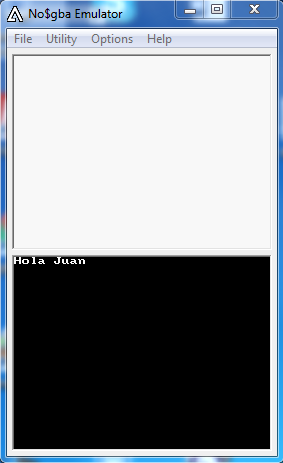
\includegraphics[height=8cm]{./Figuras/C2/c2_eclipse11b.png}
\caption{Ejecución del programa ejemplo en el emulador \textit{No\$gba}.}
\label{fig_c2_eclipse11b}
\end{figure}

Si se escoge el emulador \textit{DeSmuME}, se pulsa en \textit{File->Open ROM} y se busca el fichero \textit{.nds} que nos interesa.


% --------------------------------------------------------------------------
% --------------------------------------------------------------------------
\subsection{Desarrollar código en \textit{Linux}}
\label{sec:programa}

En esta sección se van a ver los pasos para realizar nuestro primer programa para la NDS en el sistema operativo \textit{Linux}. \textbf{En el laboratorio se debe entrar con la cuenta \textit{usuario}}. Antes de nada se debe comprobar que las siguientes variables de entorno se encuentran en el fichero \textit{.bash\_profile} del \textit{usuario}:
\begin{verbatim}
 export DEVKITPRO=/opt/devkitpro/
 export DEVKITARM=/opt/devkitpro/devkitARM/
\end{verbatim}

% --------------------------------------------------------------------------
\subsubsection{Creación de la estructura de ficheros}
Se puede emplear como punto de partida el ejemplo  \textit{hello\_world} que aparece en el directorio \textit{nds} del directorio \textit{examples} de  \textit{DevkitPro}. En  el laboratorio de prácticas, \textit{DevkitPro} se encuentra en el directorio \textit{/opt/devkitpro}. En el directorio donde se vayan a almacenar los programas a desarro\-llar se crea un nuevo directorio que identifique el programa a desarrollar (p.ej. \textit{ejemplo}). Dentro de ese directorio se crea el directorio \textit{source}, que contendrá los ficheros necesarios para el código a desarrollar (p.ej. \textit{main.c}). En el directorio \textit{ejemplo} se copia el fichero \textit{Makefile} del  ejemplo  \textit{hello\_world} de \textit{DevkitPro}. De esta forma la estructura de ficheros que se tiene es la siguiente:
\begin{verbatim}
  /home/usuario/mis_ejemplos
    - directorio ejemplo
      - fichero Makefile
      - directorio source
        - fichero main.c
\end{verbatim}

% --------------------------------------------------------------------------
\subsubsection{Edición del fichero ejemplo}
Para familiarizarse con el entorno de desarrollo de aplicaciones para Nintendo DS, se va a utilizar como ejemplo una aplicación en la que aparezca un saludo con el nombre del desarrollador del programa. Para escribir este código se puede emplear cualquier editor de texto.

Según esto, el código del programa a desarrollar (\textit{main.c}) es el siguiente:
\begin{lstlisting}
#include<nds.h>
#include<stdio.h>
int main(void)
{
	consoleDemoInit();
    iprintf("Hola Juan");  // Imprimir el mensaje 
    while(1){} // Bucle que no hace nada.     
    return 0; // Finalizar el programa
}
\end{lstlisting}

% --------------------------------------------------------------------------
\subsubsection{Compilación del fichero ejemplo}
El siguiente paso es compilar el programa, para ello se abre el \textit{Terminal} \textit{(Sistema->Terminal)}. Una vez se está en el directorio \textit{ejemplo} creado, se ejecuta el comando \textit{make}:
\begin{verbatim}
 [usuario@labsop02 ejemplo]# make
 main.c
 arm-none-eabi-gcc -MMD -MP -MF /root/mis_ejemplos/ejemplo/build/main.d -g -Wall 
 -O2 -march=armv5te -mtune=arm946e-s -fomit-frame-pointer -ffast-math 
 -mthumb -mthumb-interwork -I/root/mis_ejemplos/ejemplo/include 
 -I/root/mis_ejemplos/ejemplo/build -I/opt/devkitpro//libnds/include 
 -I/root/mis_ejemplos/ejemplo/build -DARM9 -c 
 /root/mis_ejemplos/ejemplo/source/main.c -o main.o 
 linking ejemplo.elf
 Nintendo DS rom tool 1.50.1 - Jun 19 2012
 by Rafael Vuijk, Dave Murphy, Alexei Karpenko
 built ... ejemplo.nds
\end{verbatim}

Si no se han producido errores de compilación aparecerán los ficheros \textit{ejemplo.elf} y \textit{ejemplo.nds}.
\begin{verbatim}
 [usuario@labsop02 ejemplo]# ls -l
 total 332
 drwxr-xr-x 2 root root   4096 sep  5 18:01 build
 -rwxr-xr-x 1 root root 234909 sep  5 18:01 ejemplo.elf
 -rw-r--r-- 1 root root 134208 sep  5 18:01 ejemplo.nds
 -rwxr-xr-x 1 root root   4903 abr  2  2012 Makefile
 drwxr-xr-x 2 root root   4096 sep  5 18:00 source
                \end{verbatim}
Para borrar todos los ficheros y directorios creados durante la compilación se puede ejecutar \textit{make clean}.

% --------------------------------------------------------------------------
\subsubsection{Ejecución del fichero ejemplo en el emulador}
Si no se ha producido ningún problema en la compilación, la salida del programa se puede ver en el emulador. Una vez abierto \textit{WinDS Pro}, si se escoge el emulador \textit{No\$gba}, se pulsa en \textit{File->Cartridge Menu (File Name)} y se busca el fichero \textit{.nds} que nos interesa. Si se escoge el emulador \textit{DeSmuME}, se pulsa en \textit{File->Open ROM} y se busca el fichero \textit{.nds} que nos interesa.

